% #############################################################################
% This is Chapter 4
% !TEX root = ../main.tex
% #############################################################################
% Change the Name of the Chapter i the following line
\fancychapter{Conducted Numerical Simulations}
% \cleardoublepage
% The following line allows to ref this chapter
\label{chap:implement}

Thinks to do:
\begin{enumerate}
    \item Dirac
    \begin{enumerate}
        \item Result against the ball with m=0 (accuracy)
        \item Results for quadrilaterals and Conjecture
        \item Results for triangles and Conjecture
        \item Results for smooth domains
        \item Third eigenvalue method
    \end{enumerate}
    \item Transmission
    \begin{enumerate}
        \item (WE STILL NEED PROOF!)
        \item Results against known function
        \item Results for rectangle
        \item Results for L + particular solutions
        \item Results for smooth domains
    \end{enumerate}
\end{enumerate}

\section{Dirac equation simulations}


\section{Transmission problem simulations}

For the Transmission problem, we now consider the set of equations studied previously in the subchapter \ref{domain_decomp_problem}, given by

\begin{align}\label{transmission_num}
    \begin{split}
    - \nabla k_i \nabla u_i &= f_i, \; \text{in }\Omega_i\\
    u_1 - u_2 &= 0, \; \text{on }\gamma\\
    k_1 \frac{\partial u_1}{\partial n_1} + k_2 \frac{\partial u_2}{\partial n_2} &= 0, \; \text{on }\gamma\\
    u_i &= 0, \; \text{on }\Gamma_i.
    \end{split}
\end{align}

Like before, the domain \(\Omega \subset \mathbb{R}^2\) is divided into two non-overlapping regions \(\Omega_1\) and \(\Omega_2\) such that \(\overline{\Omega} = \overline{\Omega_1} \cup \overline{\Omega_2}\). Their common boundary is denoted by \(\gamma = \partial\Omega_1 \cap \partial\Omega_2\) and the boundary of each domain (minus the common boundary) is also denoted by \(\Gamma_i = \partial\Omega_1\setminus{\gamma}\). In what follows, the source functions \(f_i\) of each domain are constant\footnote{In this work we only considered \(f_i=1\). In any case, we are still working with a general discontinuous source function (if \(k_1 \neq k_2\)). Working with different \textit{continuous} source functions should make no difference in the result. We will also present how to deal with general and continuous source functions.}, and we took \(f_i = 1\). Recall that \(k_1 \geq k_2 > 0\) are constants and \(n_i\) is the (normalized) outward normal to each domain subdomain \(\Omega_i, i=1, 2\), where we shall write \(n=n_1=-n_2\) when we are restricted to the interface.

The procedure presented here is based on \cite{alves2005new} and \cite{alves2021domain}. Given that \(f_i = 1\) for each \(i=1, 2\), a solution of \eqref{transmission_num} can be found by taking the following steps:
\begin{enumerate}
    \item Find a solution for the non-homogeneous problem
    \[
        \begin{cases}
            -\Delta u_1^{NH} = \frac{1}{k_1}\\
            -\Delta u_2^{NH} = \frac{1}{k_2}.
        \end{cases}
    \]
    This can easily be done, and we have
    \[
        \begin{cases}
            u_1^{NH} = -\frac{x_1^2 + x_2^2}{4k_1}\\
            u_2^{NH} = -\frac{x_1^2 + x_2^2}{4k_2};
        \end{cases}
    \]
    \item Then we solve the homogeneous problem
    \begin{align}\label{transmission_num_homo}
        \begin{split}
        - \nabla k_i \nabla u_i^H &= 0, \; \text{in }\Omega_i\\
        u_1^H - u_2^H &= u_2^{NH}- u_1^{NH}, \; \text{on }\gamma\\
        k_1 \frac{\partial u_1}{\partial n_1} + k_2 \frac{\partial u_2}{\partial n_2} &= u_2^{NH} - u_1^{NH}, \; \text{on }\gamma\\
        u_i &= - u_i^{NH}, \; \text{on }\Gamma_i;
        \end{split}
    \end{align}
    \item Finally, the solution of \eqref{transmission_num} is \(u_i = u_i^H + u_i^{NH}\).
\end{enumerate}
For general source functions, the steps above can also be used: however, it may not be possible to find an analytical solution in first step. In this case, \textbf{1.} must be solved numerically. A popular choice is to use radial basis functions (RBFs) (see \cite{golberg1996improved} for example), like the thin plate spline
\[
    \varphi(r) = r^2 \log r,     
\]
and find the coefficients \(\alpha_j\) in \(f_i(x_k) = \tilde{f}_i(x_k) = \sum_{j=1}^{n} \alpha_j \varphi_j(x_k)\) using least square methods, where \(x_k\) are collocation points. Finally, one can analytically solve the equation \(-\Delta \Psi_j = \varphi_j\) to recover the non-homogeneous solutions \(u_1^{NH}\) and \(u_2^{NH}\). In \cite{alves2005new} and \cite{alves2021domain} a different approach was suggested using the fundamental solutions of the Helmholtz equation instead of the classical RBFs; that method is known today as \textit{Kansa MFS method}.

In what follows, the numerical results illustrate the accuracy of the method in simply connected 2D domains. Let \(N_i\) denote the number of source points for each domain \(i\), such that \(N=N_1+N_2\). We denote the approximate solution by
\[
    \tilde{u} = \begin{cases}
        \tilde{u}_1, & \text{in } \Omega_1\\
        \tilde{u}_2, & \text{in } \Omega_2,
    \end{cases}
\]
where
\begin{align*}
    &\tilde{u}_1(x) = \sum_{j=1}^{N_1} \alpha^{(1)}_j \Phi\left(x-y_j^{(1)}\right)\\
    &\tilde{u}_2(x) = \sum_{j=1}^{N_2} \alpha^{(2)}_j \Phi\left(x-y_j^{(1)}\right).
\end{align*}
Let \(M_i\) be the number of boundary collocation points \(x^{(i)}_{m}\) for each \(\Omega_i\) and \(M=M_1+M_2\). We also consider \(Q\) interface points \(z_q \in \gamma\) with \(q=1,\dots,Q\). Then, a full block system is written as
\begin{equation}\label{mfs_transmission_classical_matrices_system}
    \renewcommand{\arraystretch}{1.75} % Increase spacing between rows of the matrices
    \begin{bmatrix}
        \left[\Phi\left(x^{(1)}_{m}-y_j^{(1)}\right)\right] & [0] \\
        [0] & \left[\Phi\left(x^{(2)}_{m}-y_j^{(2)}\right)\right] \\
        \left[\Phi\left(z_q-y_j^{(1)}\right)\right] & \left[-\Phi\left(z_q-y_j^{(2)}\right)\right] \\
        \left[k_1\partial_n \Phi\left(z_q-y_j^{(1)}\right)\right] & \left[-k_2 \partial_n \Phi\left(z_q-y_j^{(2)}\right)\right]
    \end{bmatrix}
    \begin{bmatrix}
        \left[\alpha^{(1)}_j\right]\\
        \left[\alpha^{(2)}_j\right]
    \end{bmatrix}=
    \begin{bmatrix}
        \left[-u_1^{NH}(x^{(1)}_{m})\right]\\
        \left[-u_2^{NH}(x^{(2)}_{m})\right]\\
        \left[u_2^{NH}(z_q)-u_1^{NH}(z_q)\right]\\
        \left[k_2 \partial_n u_2^{NH}(z_q)- k_1 \partial_n u_1^{NH}(z_q)\right]\\
    \end{bmatrix}
\end{equation}

Most of the examples below do not have analytical solution: only in the subsection \ref{transmission_val_subsection}, when we test the results against a known solution, we are able to find the absolute error. In the other cases we are only interested in the relative error, i.e, the boundary error (against which we can compare since \(u_i=0\) in \(\Gamma_i\)) and the interface error by checking the transmission conditions on \(\gamma\):
\begin{itemize}
    \item \(\norm*{\tilde{u}_i - 0}_{L^2(\Gamma_i)}\), \(i=1, 2\): boundary collocation error;
    \item \(\norm*{\tilde{u}_1 - \tilde{u}_2}_{L^2(\gamma)}\), \(i=1, 2\): continuity error (\(C^0\)) of \(\tilde{u}\) across \(\gamma\);
    \item \(\norm*{k_1 \partial_n\tilde{u}_1 - k_2 \partial_n\tilde{u}_2}_{L^2(\gamma)}\), \(i=1, 2\): continuity error \(C^1\) of \(\partial_n\tilde{u}\) across \(\gamma\).
\end{itemize}
From a numerical point of view, let \(\mathcal{I}\) be the sample of test points. The \(L^2\) norm is discretized into the Root Mean Squared Error (RMSE) which is equivalent to the \(l^2\) norm and is given by
\[
    \norm*{u-\tilde{u}}= \sqrt{\frac{1}{\#\mathcal{I}} \sum_{z \in \mathcal{I}} \abs{u(z)-\tilde{u}(z)}^2}.
\]
For every result below the number of sample test points is 5 times larger than the sample used to find the coefficients of the MFS. 

\subsection{Numerical validation of the method}\label{transmission_val_subsection}

First, we start by testing the numerical algorithm for the unit disk \(\mathbb{D}\), with \(k_1=k_2=1\). From Theorem \eqref{equivalence_transmission}, we know that the system of differential equations \eqref{transmission_num} is equivalent to the Poisson equation
\begin{align}\label{transmission_disk}
    \begin{split}
        -\Delta u = 1, & \text{ in } \mathbb{D}\\
        u = 0, & \text{ on } \partial\mathbb{D},
    \end{split}
\end{align}
and is easy so see that the exact solution of Equation \eqref{transmission_disk} is given in polar coordinates by \(u(r, \theta) = \frac{1-r^2}{4}\). 

\begin{figure}[!htb]
    \centering
    \begin{minipage}{.5\textwidth}
      \centering
      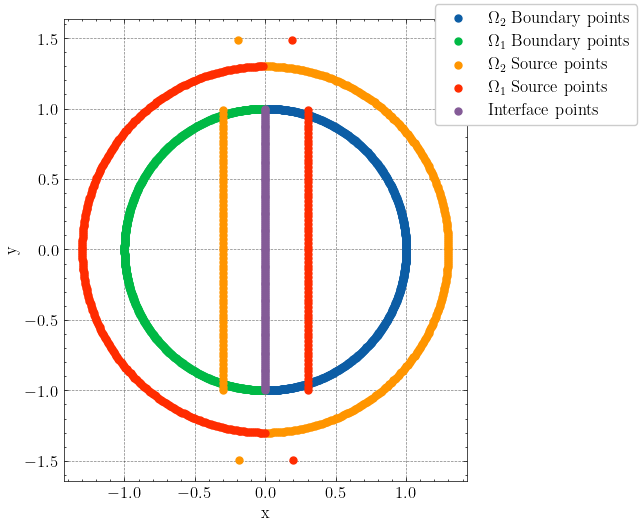
\includegraphics[width=1\linewidth]{Images/Transmission/Circle_val_col_points_600_150.png}
      \captionsetup{width=0.9\linewidth} % Adjust the width of the caption
      \captionof{figure}{Configuration of the boundary, source and interface points. Each domain has 600 boundary points, 377 source points and the common interface has 100 points.}
      \label{transmission_disk_col}
    \end{minipage}%
    %\hspace{0.5cm} % Add some horizontal space between the figures
    \begin{minipage}{.5\textwidth}
      \centering
      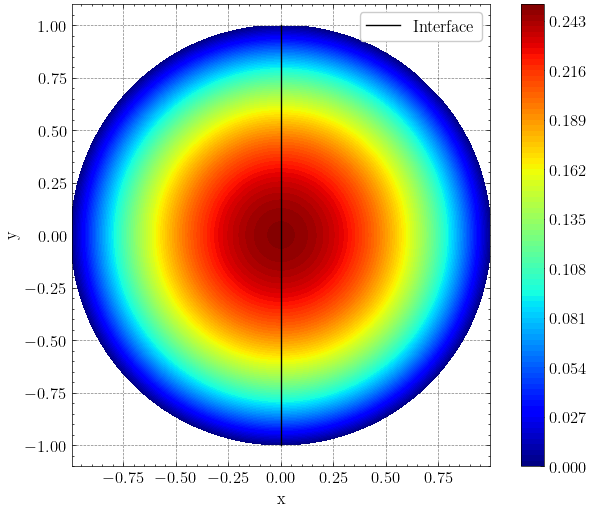
\includegraphics[width=1\linewidth]{Images/Transmission/Circle_val_contour_600_150.png}
      \captionsetup{width=0.9\linewidth} % Adjust the width of the caption
      \captionof{figure}{Numerical approximation of the BVP \eqref{transmission_disk} under the conditions presented in Figure \ref{transmission_disk_col}}
      \label{transmission_disk_plot}
    \end{minipage}
\end{figure}

The absolute error between the approximate solution and the exact solution can then be calculated for each domain point. The sample points to compute the absolute error were generated in a uniform grid and were also used to plot Figure \ref{transmission_disk_plot}. The method described at the end of the subchapter \ref{density_proofs_section} was used to place the source points, where \(\eta=0.3\).

\begin{table}[htbp]
    \centering
    \begin{tabular}{cccccc}
        \toprule
        \multirow{2}{*}{\textbf{Boundary/Interface Points}} & \multicolumn{2}{c}{\textbf{Boundary Error}} & \multicolumn{2}{c}{\textbf{Absolute Error}} \\
        \cmidrule(lr){2-3} \cmidrule(lr){4-5}
        & \textbf{Domain 1} & \textbf{Domain 2} & \textbf{Domain 1} & \textbf{Domain 2} \\
        \midrule
        600/150 & $9.759\times10^{-12}$ & $9.541\times10^{-12}$ & $1.465\times10^{-11}$ & $1.439\times10^{-11}$ \\
        500/100 & $3.667\times10^{-11}$ & $3.945\times10^{-11}$ & $9.382\times10^{-11}$ & $9.310\times10^{-11}$ \\
        412/100 & $3.721\times10^{-11}$ & $5.036\times10^{-11}$ & $9.652\times10^{-11}$ & $9.584\times10^{-11}$ \\
        \bottomrule
    \end{tabular}
    \caption{Numerical errors for the boundary and the whole Domains \(\Omega_1\) and \(\Omega_2\)}
    \label{tab:transmission_results_1}
\end{table}


\begin{table}[htbp]
    \centering
    \begin{tabular}{cccc}
      \toprule
      \textbf{Boundary/Interface Points} & \textbf{Interface \(C^0\) Error} & \textbf{Interface \(C^1\) Error} & \textbf{Condition number} \\
      \midrule
      600/150 & $6.945\times10^{-11}$ & $1.841\times10^{-11}$ & $2.528\times 10^{19}$\\
      500/100 & $3.910\times10^{-10}$ & $1.100\times10^{-10}$ & $2.382\times 10^{18}$\\
      412/100 & $4.035\times10^{-10}$ & $1.342\times10^{-10}$ & $7.597\times 10^{17}$\\
      \bottomrule
    \end{tabular}
    \caption{Numerical error on the interface \(\gamma\). The condition number of the matrix is also presented.}
    \label{tab:transmission_results_2}
\end{table}

The numerical results presented in Tables \ref{tab:transmission_results_1} and \ref{tab:transmission_results_2} are not yet optimal. When considering a larger value of \(\eta\), the results increase by more than two orders of magnitude, but this also leads to a significant increase in the already very high condition number (see Table \ref{tab:transmission_results_2}), as expected. Despite this, the results show great promise, which was anticipated due to the analyticity of the domain.

As mentioned previously, the Method of Fundamental Solutions (MFS) yields better results in highly regular domains, even when considering curved geometries. However, increasing the number of boundary and interface collocation points improves the accuracy of the solution. It is important to note that a larger number of points also escalates the condition number, making the problem more challenging to solve accurately.

The inclusion of the ``corner'' source points, as depicted in Figure \ref{transmission_disk_col}, also significantly impacts the method's accuracy. These source points above and below the interface (\ref{transmission_disk_col}) are strategically added, in order to capture the behavior near the interface corner. In Figure \ref{transmission_disk_col}, observe that the source points for one of the domains can be inside the other domain, as the solution will be split into two parts.

\subsection{Results for the rectangle}

In this subsection a rectangular domain \([-1, -0.5] \times [1, 0.5]\) with a vertical interface along the line \(x=0\) is considered. We are now interested to study the problem for \(k_1 \neq k_2\) where \(k_2=1\) is fixed. The results below were conducted with 600 boundary points and 404 source points for each domain. The number of interface points is 150 and \(\eta=0.08\).

\begin{figure}[!htb]
    \centering
    \begin{minipage}{.5\textwidth}
      \centering
      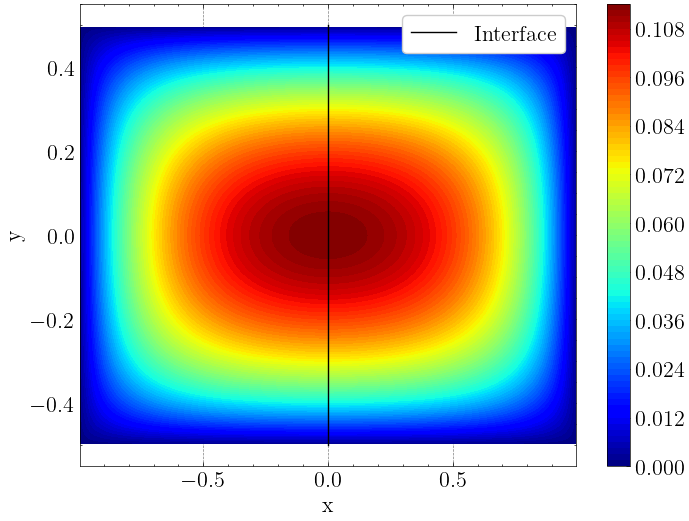
\includegraphics[width=\linewidth]{Images/Transmission/Rectangle_contour_600_150_k1_1.png}
      \caption{Numerical simulation with  \(k_1=1\).}
      \label{transmission_rectangle_plot_k1_1}
    \end{minipage}%
    \begin{minipage}{.5\textwidth}
      \centering
      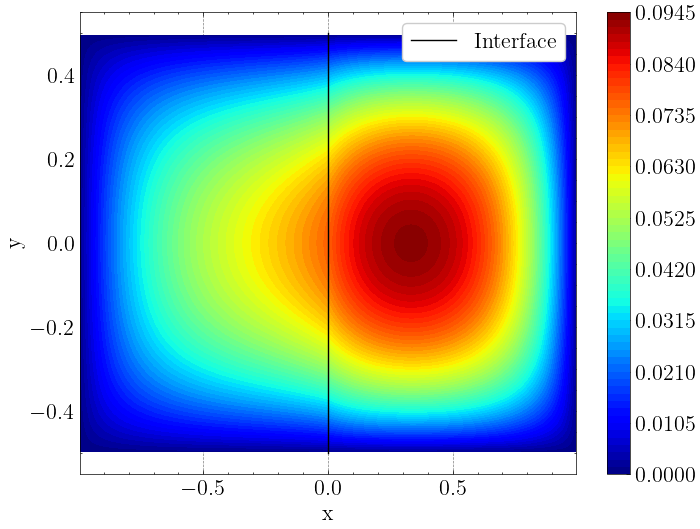
\includegraphics[width=\linewidth]{Images/Transmission/Rectangle_contour_600_150_k1_2.png}
      \caption{Numerical simulation with \(k_1=2\).}
      \label{transmission_rectangle_plot_k1_2}
    \end{minipage}
    
    \vspace{0.5cm} % Add some vertical space between the rows of figures
    
    \begin{minipage}{.6\textwidth}
      \centering
      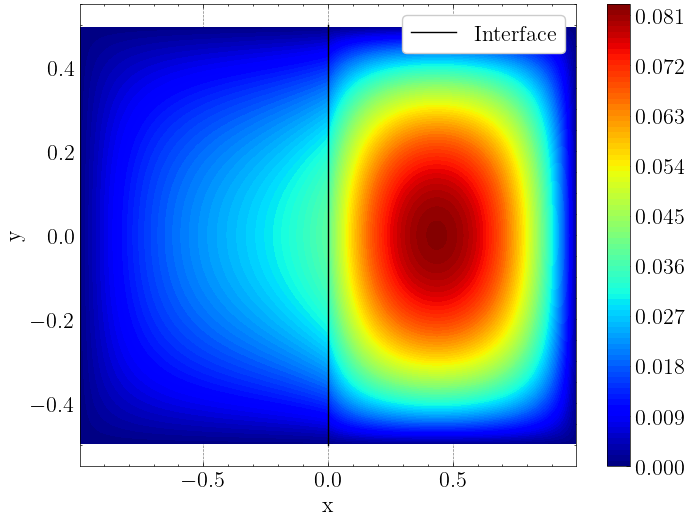
\includegraphics[width=\linewidth]{Images/Transmission/Rectangle_contour_600_150_k1_5.png}
      \caption{Numerical simulation with  \(k_1=5\).}
      \label{transmission_rectangle_plot_k1_5}
    \end{minipage}
    
    \caption*{Numerical approximations of the BVP for a rectangular domain with different \(k_1\) values.}
    \label{transmission_rectangle_plots}
\end{figure}

\begin{table}[htbp]
    \centering
    \begin{tabular}{cccccc}
      \toprule
      \multirow{2}{*}{\textbf{\(k_1\) value}} & \multicolumn{2}{c}{\textbf{Boundary Error}} & \multicolumn{2}{c}{\textbf{Interface Errors}} & \multirow{2}{*}{\textbf{Condition number}} \\
      \cmidrule(lr){2-3} \cmidrule(lr){4-5}
      & \textbf{Domain 1} & \textbf{Domain 2} & \textbf{\(C^0\)} & \textbf{\(C^1\)} & \\
      \midrule
      1 & $7.775\times10^{-8}$ & $7.779\times10^{-8}$ & $4.732\times10^{-9}$ & $7.589\times10^{-9}$ & $2.331\times 10^{13}$\\
      2 & $4.398\times10^{-8}$ & $8.614\times10^{-8}$ & $2.499\times10^{-6}$ & $7.868\times10^{-8}$ & $3.623\times 10^{13}$\\
      3 & $2.181\times10^{-8}$ & $1.036\times10^{-7}$ & $3.838\times10^{-6}$ & $1.551\times10^{-7}$ & $8.182\times 10^{13}$\\
      \bottomrule
    \end{tabular}
    \caption{Numerical error on the interface \(\gamma\). The condition number of the matrix is also presented.}
    \label{tab:transmission_results_rectangle}
\end{table}

In Figures \ref{transmission_rectangle_plot_k1_1}, \ref{transmission_rectangle_plot_k1_2} and \ref{transmission_rectangle_plot_k1_5} we present the numerical approximation for different \(k_1\) values. Observe that increasing \(k_1\) breaks the symmetry of the solution which shifts from \(\Omega_1\) (the domain on the left) and \(\Omega_2\) (the domain on the right). Table \ref{tab:transmission_results_rectangle} summarizes the results for different \(k_1\) values. While the results are slightly worst that the previous ones due to the worst domain regularity, they still preserve high accuracy. It is worth to remark that for different values of \(k_1\) and \(k_2\) decreases the accuracy of the method. This is also to be expected, since we are dealing with a discontinuous source function which decreases the regularity of the solution. 

Notice that the condition number for the rectangle is smaller than the one presented in Table \ref{tab:transmission_results_2} for the unit disk. This is a consequence of a smaller value of \(\eta\), which in this case appears to be optimal, since increasing its value decreases the overall accuracy. 

\subsection{Results for an L-shape domain with enrichment}

In the previous subsection a domain with corners was analyzed. However, it still preserved some regularity and the MFS with classical basis functions was able to capture its corner's behavior, as explained in Remark \ref{particular_solutions}. In what follows, we are going to study the case of an L-shape, a non-convex domain with singular corners. Two different interfaces will be considered: first, the usual interface along the line \(x=0\); then, along its symmetry axis with the line \(y=\frac{1}{2}x\).

Consider the L-shape given in Figure \ref{transmission_L_shape_config}. The left and the right subdomains are \(\Omega_1\) and \(\Omega_2\), respectively. Again, the number of interface points is 150 and the number of source points for each domain is 428. The number of boundary collocation points for \(\Omega_1\) and \(\Omega_2\) are 710 and 639, respectively. 

\begin{figure}[!htb]
        \centering
        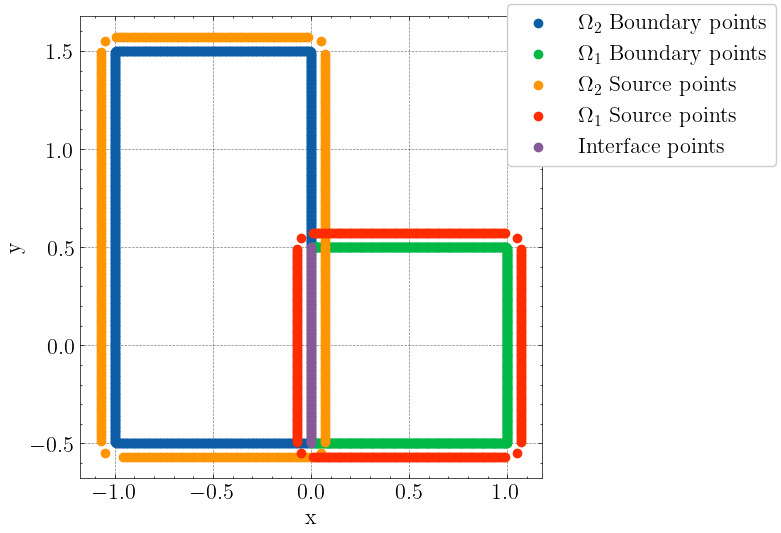
\includegraphics[width=0.5\linewidth]{Images/Transmission/L_shape_2_rectangles_col_points.png}
        \caption{L-shape domain with vertical interface. Configuration of the boundary, source and interface points.}
        \label{transmission_L_shape_config}
\end{figure}

In Table \ref{tab:transmission_results_L_shape_rectangles}, the results without resorting to enrichment are presented. It is evident that the method yields poorer results due to the lower regularity of the domain. Particularly, the interface error (mainly the \(C^0\) error) is significantly higher compared to previous cases. In fact, it appears that the domain itself poses more challenges than the discontinuous source function when considering different values for \(k_1\) and \(k_2\). In Figure \ref{transmission_L_shape_k1_5} it is even possible to see that already exists some small jump near the edges of the interface.

\begin{figure}[!htb]
    \centering
    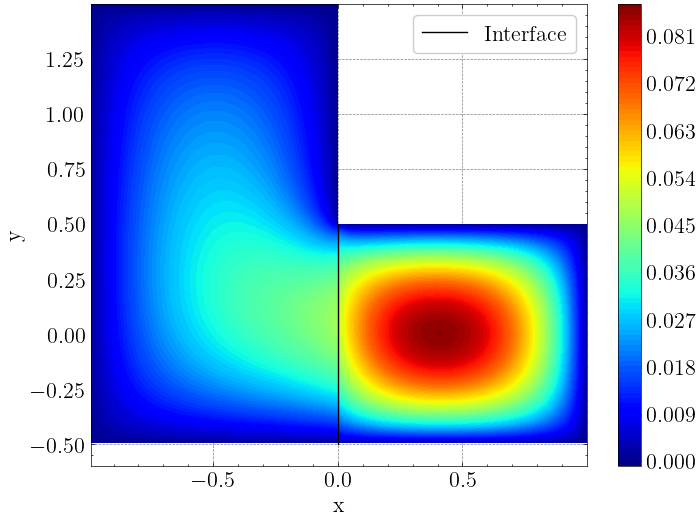
\includegraphics[width=0.7\linewidth]{Images/Transmission/L_shape_2_rectangles_k1_5.png}
    \caption{Numerical approximation of the BVP for an L-shape domain with interface along \(x=0\) and \(k_1=5\).}
    \label{transmission_L_shape_k1_5}
\end{figure}

\begin{table}[htbp]
    \centering
    \begin{tabular}{cccccc}
      \toprule
      \multirow{2}{*}{\textbf{\(k_1\) value}} & \multicolumn{2}{c}{\textbf{Boundary Error}} & \multicolumn{2}{c}{\textbf{Interface Errors}} & \multirow{2}{*}{\textbf{Condition number}} \\
      \cmidrule(lr){2-3} \cmidrule(lr){4-5}
      & \textbf{Domain 1} & \textbf{Domain 2} & \textbf{\(C^0\)} & \textbf{\(C^1\)} & \\
      \midrule
      1 & $7.057\times10^{-5}$ & $1.156\times10^{-4}$ & $2.686\times10^{-3}$ & $8.639\times10^{-5}$ & $4.020\times 10^{12}$ \\
      2 & $7.173\times10^{-5}$ & $1.372\times10^{-4}$ & $3.766\times10^{-3}$ & $2.881\times10^{-5}$ & $5.799\times 10^{12}$ \\
      3 & $7.228\times10^{-5}$ & $1.245\times10^{-4}$ & $3.473\times10^{-3}$ & $3.403\times10^{-4}$ & $1.256\times 10^{13}$ \\
      \bottomrule
    \end{tabular}
    \caption{Numerical error on the interface \(\gamma\). The condition number of the matrix is also presented.}
    \label{tab:transmission_results_L_shape_rectangles}
\end{table}

One of the major problems for the method is the behavior of the solution near the degenerate corner with \(\pi\) radians in \(\Omega_1\), where some singularity may exist due to the different boundary conditions imposed there. Notice that for \(\Omega_2\) there exists no problem since the interface edge makes a right angle with the adjacent edges. Therefore, we consider some particular solutions which describe the solution in the domain \(\Omega_1\). In this case, we are going to use Dirichlet-Neummann particular solutions, like the ones presented in \ref{m_particular_solutions}, centered in the singular corner. Let
\begin{equation}\label{pat_sol_L_shape_rect}
    v_k(r, \theta) = \alpha_k r^{\alpha_k} \sin(\alpha_k(\theta - \theta_1))
\end{equation}
where
\[
    \alpha_k = \frac{k+\frac{1}{2}\pi}{\Theta},
\]
\(\theta_1 = \frac{\pi}{2}\) is the angle shift, \(\Theta = \pi\) is the total angle amplitude,  and the coordinates \(r\) and \(\theta\) are given in polar coordinates by
\[
    r(x,y) = \sqrt{x^2+y^2} \quad \theta(x,y)=\begin{cases}
        \arctan(\frac{y}{x}),& \text{if} \arctan(\frac{y}{x})>0\\
        \arctan(\frac{y}{x})+2\pi,& \text{if} \arctan(\frac{y}{x})\leq0.
    \end{cases}
\]
By differentiating Equation \eqref{pat_sol_L_shape_rect} in cartesian coordinates and substituting polar coordinates again we find that
\begin{equation*}
    \nabla v_k(r, \theta) = \left(-\frac{(2 \pi  k+\pi )^2 r^{\frac{2 \pi  k+\pi }{2 \Theta }} \sin \left(\theta +\frac{\pi  \left(k+\frac{1}{2}\right) (s-\theta )}{\Theta }\right)}{4 \Theta ^2 r},\frac{(2 \pi  k+\pi )^2 r^{\frac{2 \pi  k+\pi }{2 \Theta }} \cos \left(\theta +\frac{\pi  \left(k+\frac{1}{2}\right) (s-\theta )}{\Theta }\right)}{4 \Theta ^2 r}\right).
\end{equation*}
Finally, considering the truncated expansion
\[
    \phi(r,\theta)=\sum_{k=1}^{P} \beta_k v_k(r, \theta),
\]
and expanding the matrix in \eqref{mfs_transmission_classical_matrices_system}, one can write
\begin{align*}
    \renewcommand{\arraystretch}{1.75} % Increase spacing between rows of the matrices
    \begin{bmatrix}
        \left[\Phi\left(x^{(1)}_{m}-y_j^{(1)}\right)\right] & [0] & \left[\phi(r\left(x_m\right),\theta\left(x_m\right))\right]\\
        [0] & \left[\Phi\left(x^{(2)}_{m}-y_j^{(2)}\right)\right] & \left[0\right]\\
        \left[\Phi\left(z_q-y_j^{(1)}\right)\right] & \left[-\Phi\left(z_q-y_j^{(2)}\right)\right] & \left[\phi(r\left(z_k\right),\theta\left(z_q\right))\right]\\
        \left[k_1\partial_n \Phi\left(z_q-y_j^{(1)}\right)\right] & \left[-k_2 \partial_n \Phi\left(z_q-y_j^{(2)}\right)\right] & \left[k_1 \partial_n\phi(r\left(x_m\right),\theta\left(x_m\right))\right]
    \end{bmatrix}
    \begin{bmatrix}
        \left[\alpha^{(1)}_j\right]\\
        \left[\alpha^{(2)}_j\right]\\
        \left[\beta_k\right]
    \end{bmatrix}=\\
    \renewcommand{\arraystretch}{1.75} % Increase spacing between rows of the matrices
    \begin{bmatrix}
        \left[-u_1^{NH}(x^{(1)}_{m})\right]\\
        \left[-u_2^{NH}(x^{(2)}_{m})\right]\\
        \left[u_2^{NH}(z_q)-u_1^{NH}(z_q)\right]\\
        \left[k_2 \partial_n u_2^{NH}(z_q)- k_1 \partial_n u_1^{NH}(z_q)\right]\\
    \end{bmatrix}
\end{align*}


\subsection{Results for the smooth domains}
